% Auto-generated by HPGCS_graphs_and_diagrams.ipynb
% Include in paper with: \input{paper/figures_auto.tex}

% Figure 1
egin{figure}[t]
\centering
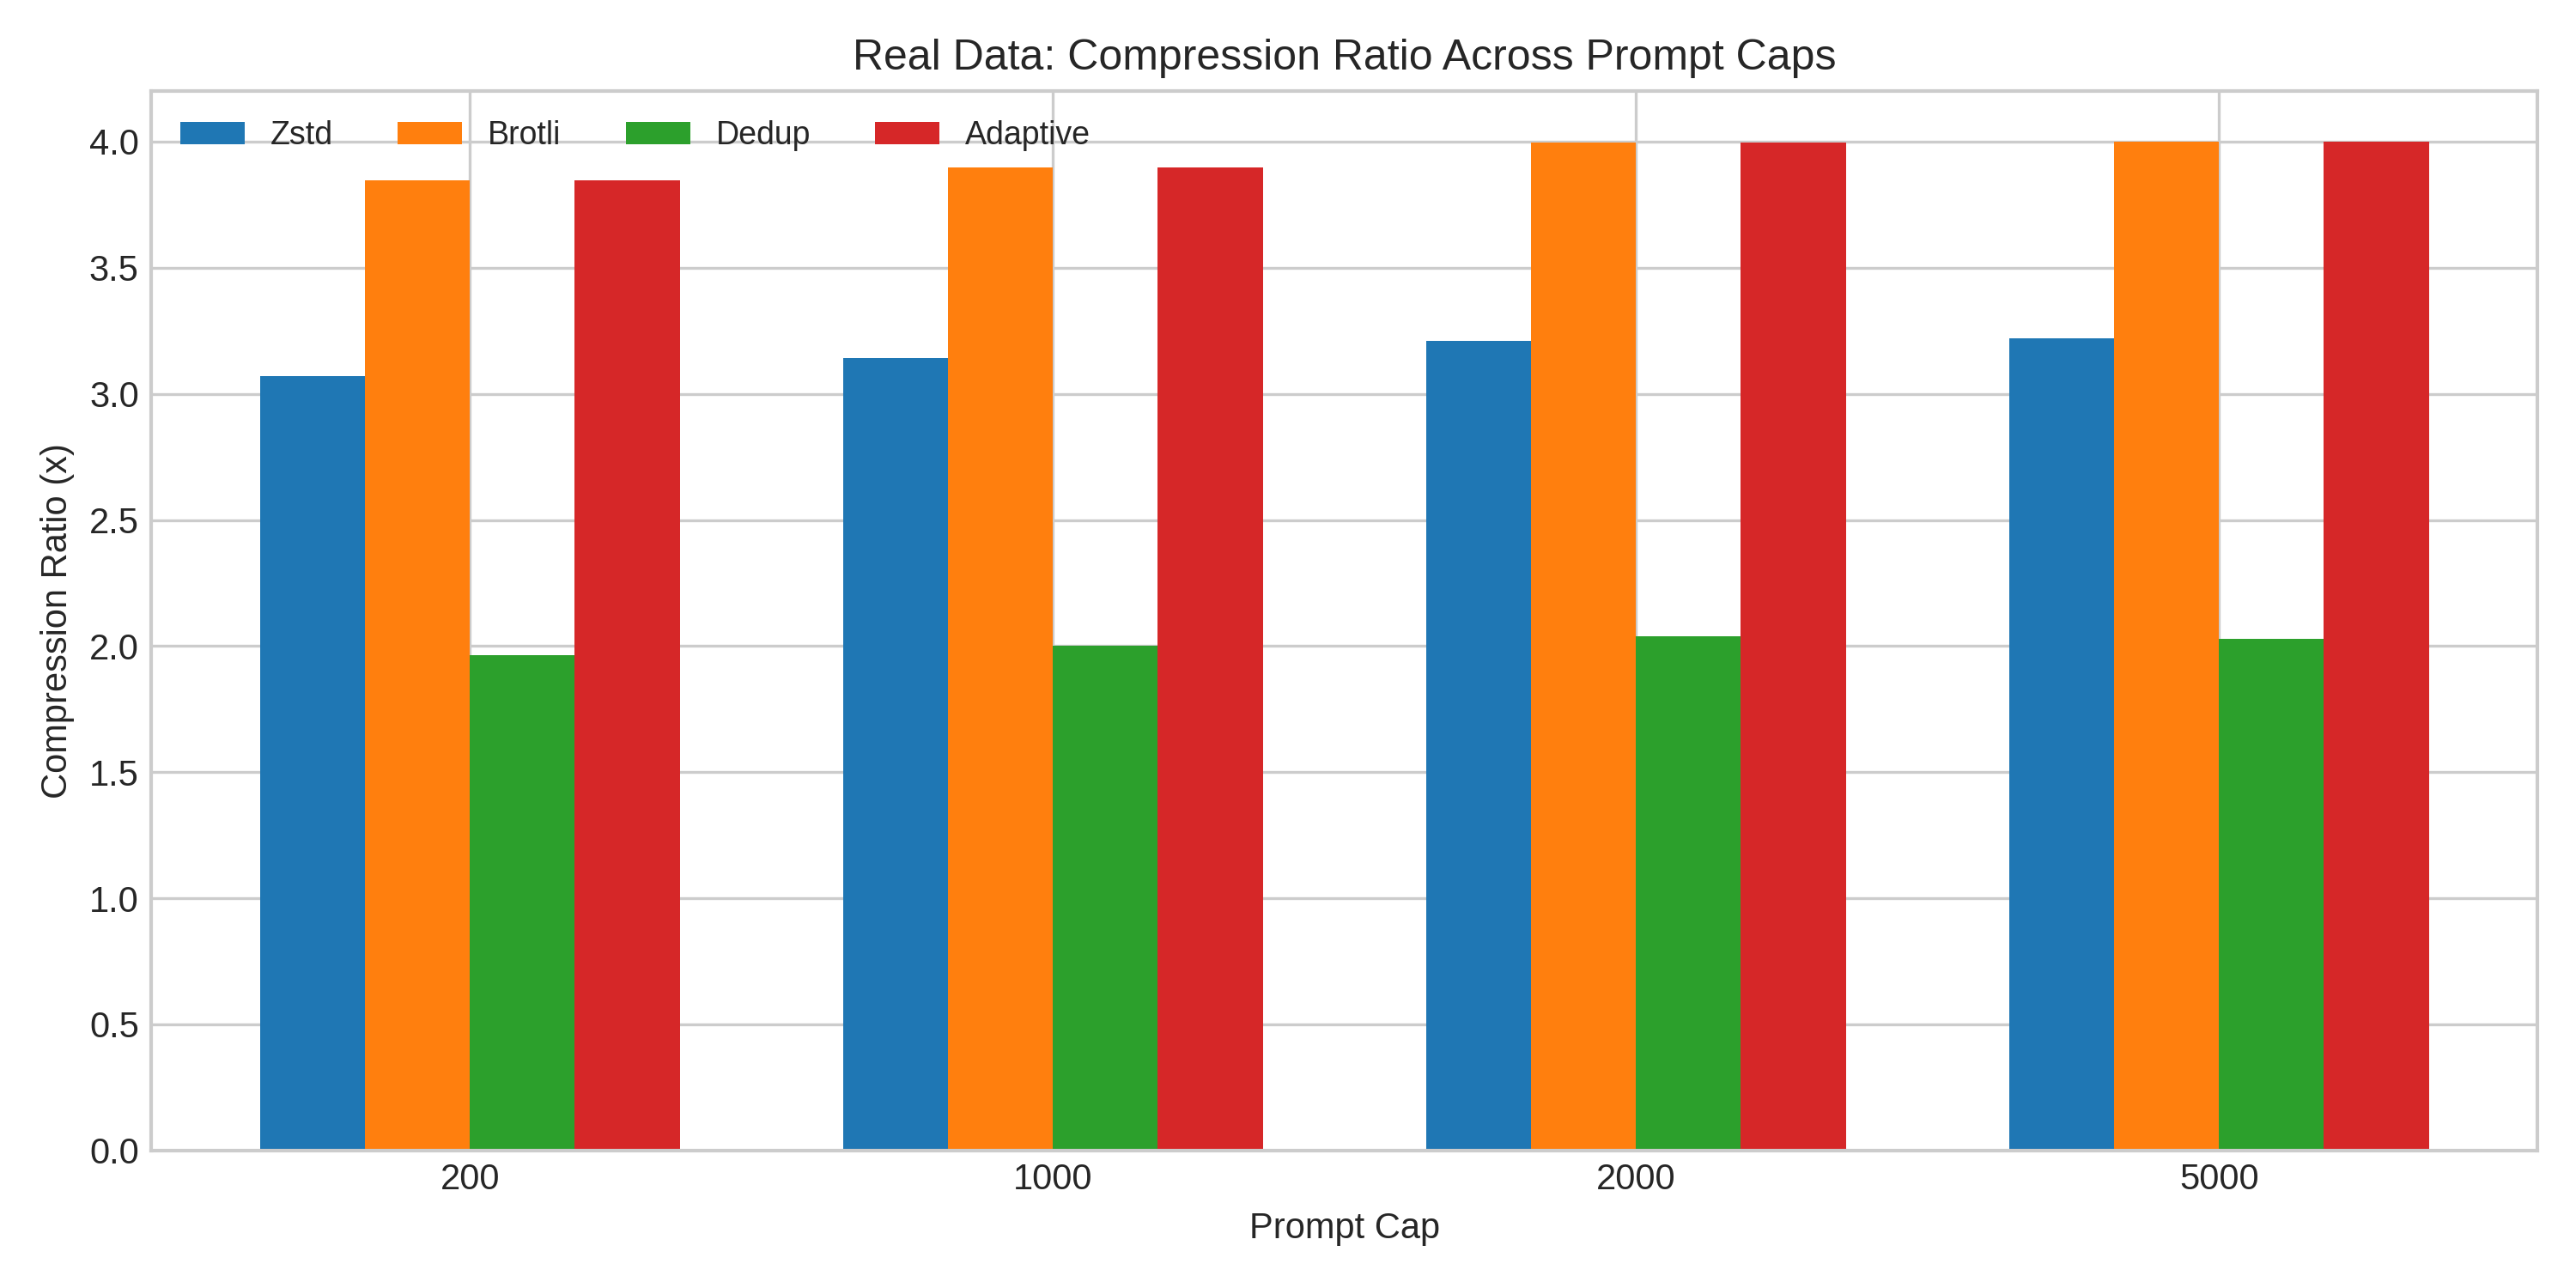
\includegraphics[width=\linewidth]{paper/figures/fig1_real_caps_ratio.png}
\caption{Fig1 Real Caps Ratio}
\label{fig:auto_fig1_real_caps_ratio}
\end{figure}

% Figure 2
egin{figure}[t]
\centering
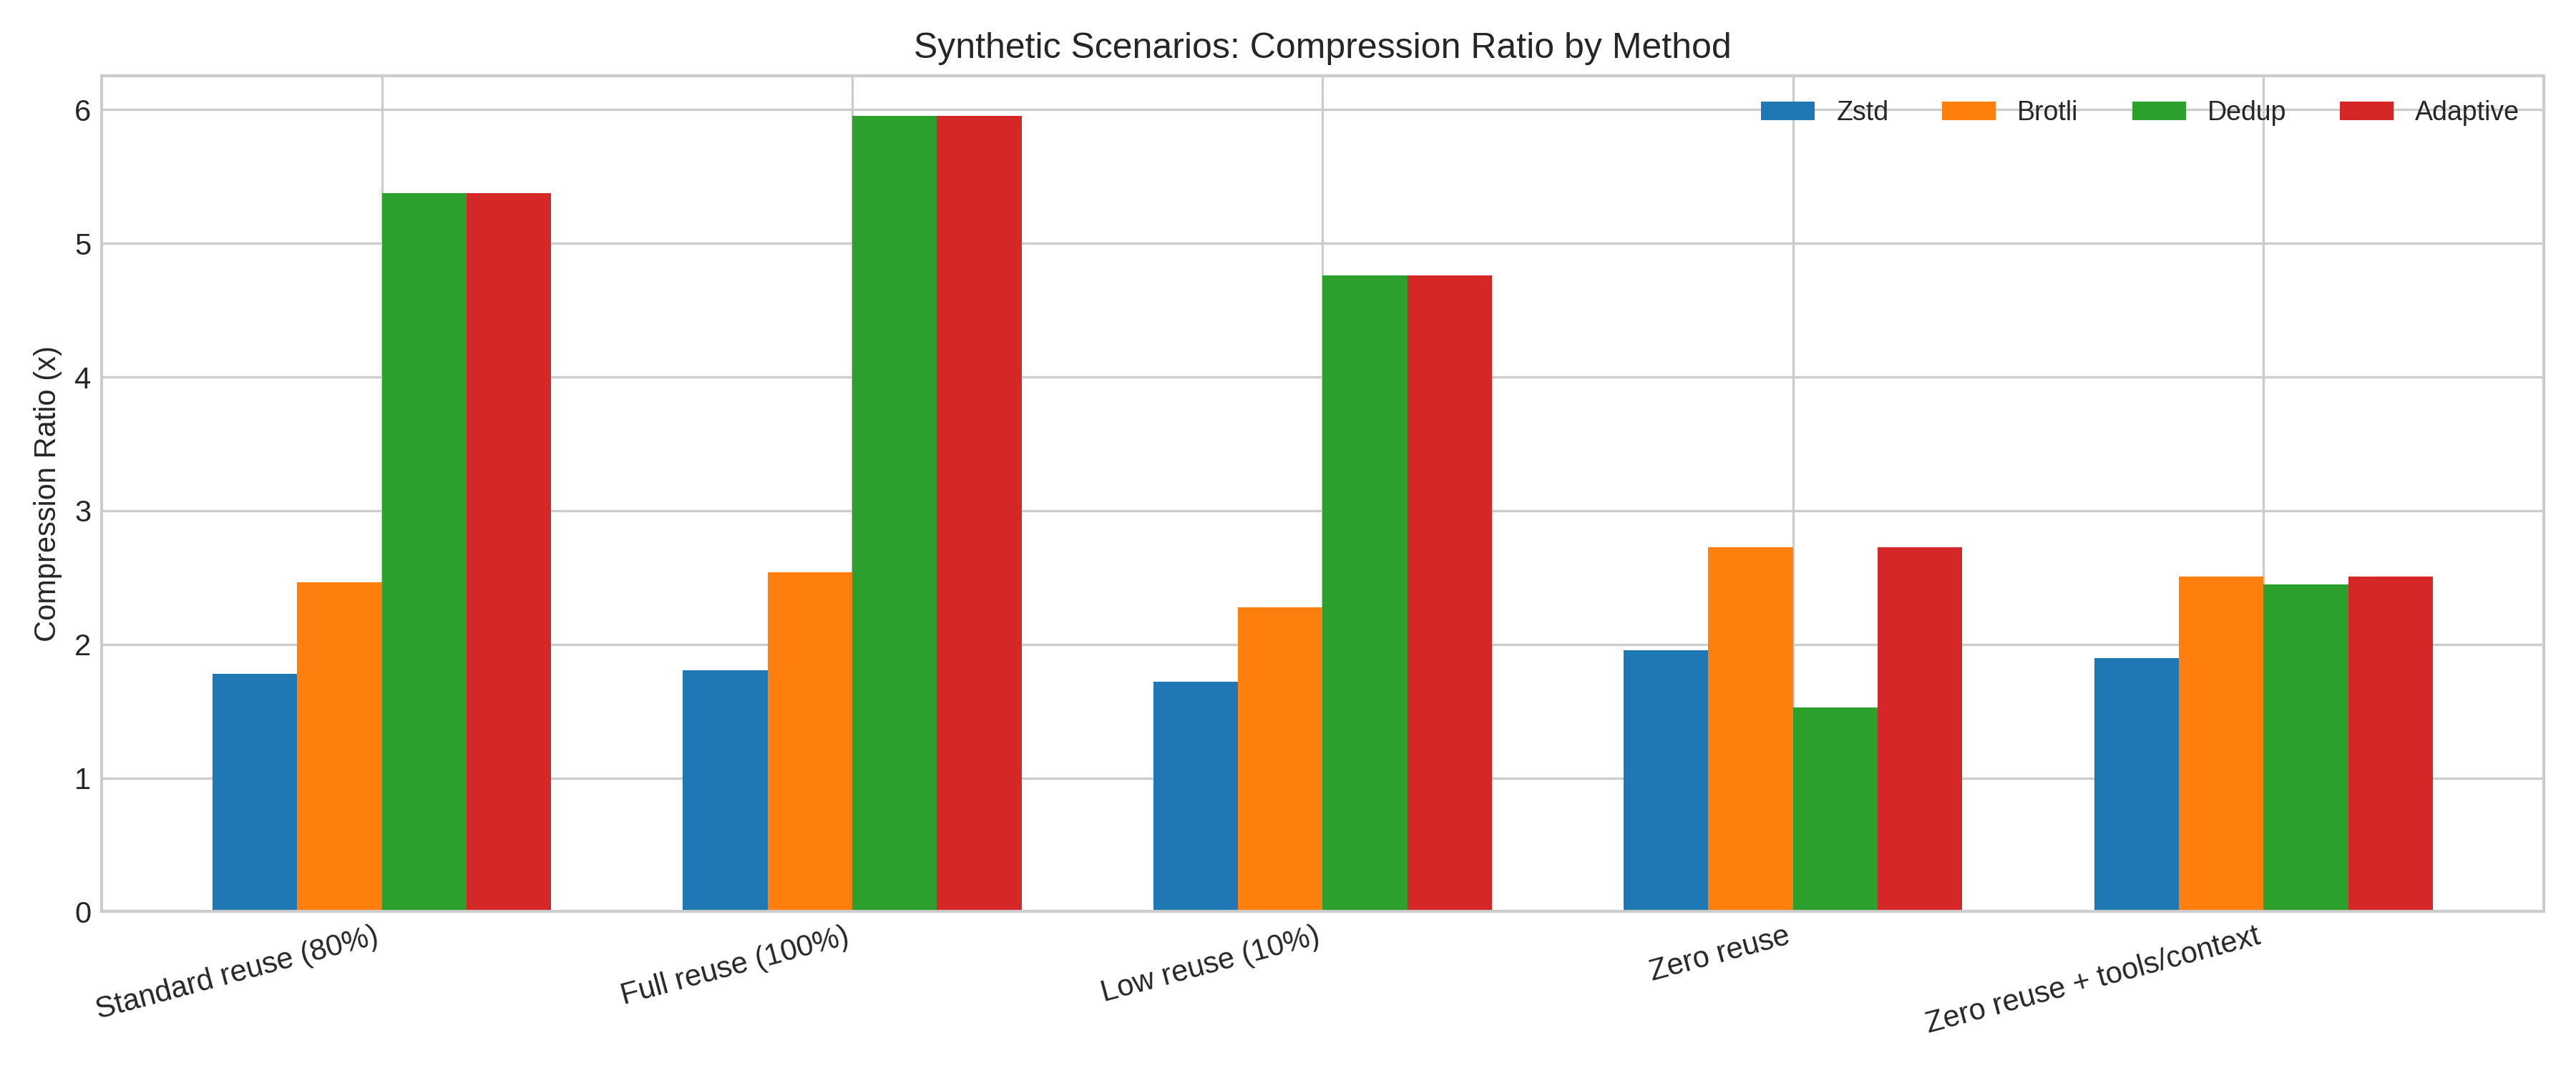
\includegraphics[width=\linewidth]{paper/figures/fig2_synthetic_scenarios_ratio.png}
\caption{Fig2 Synthetic Scenarios Ratio}
\label{fig:auto_fig2_synthetic_scenarios_ratio}
\end{figure}

% Figure 3
egin{figure}[t]
\centering
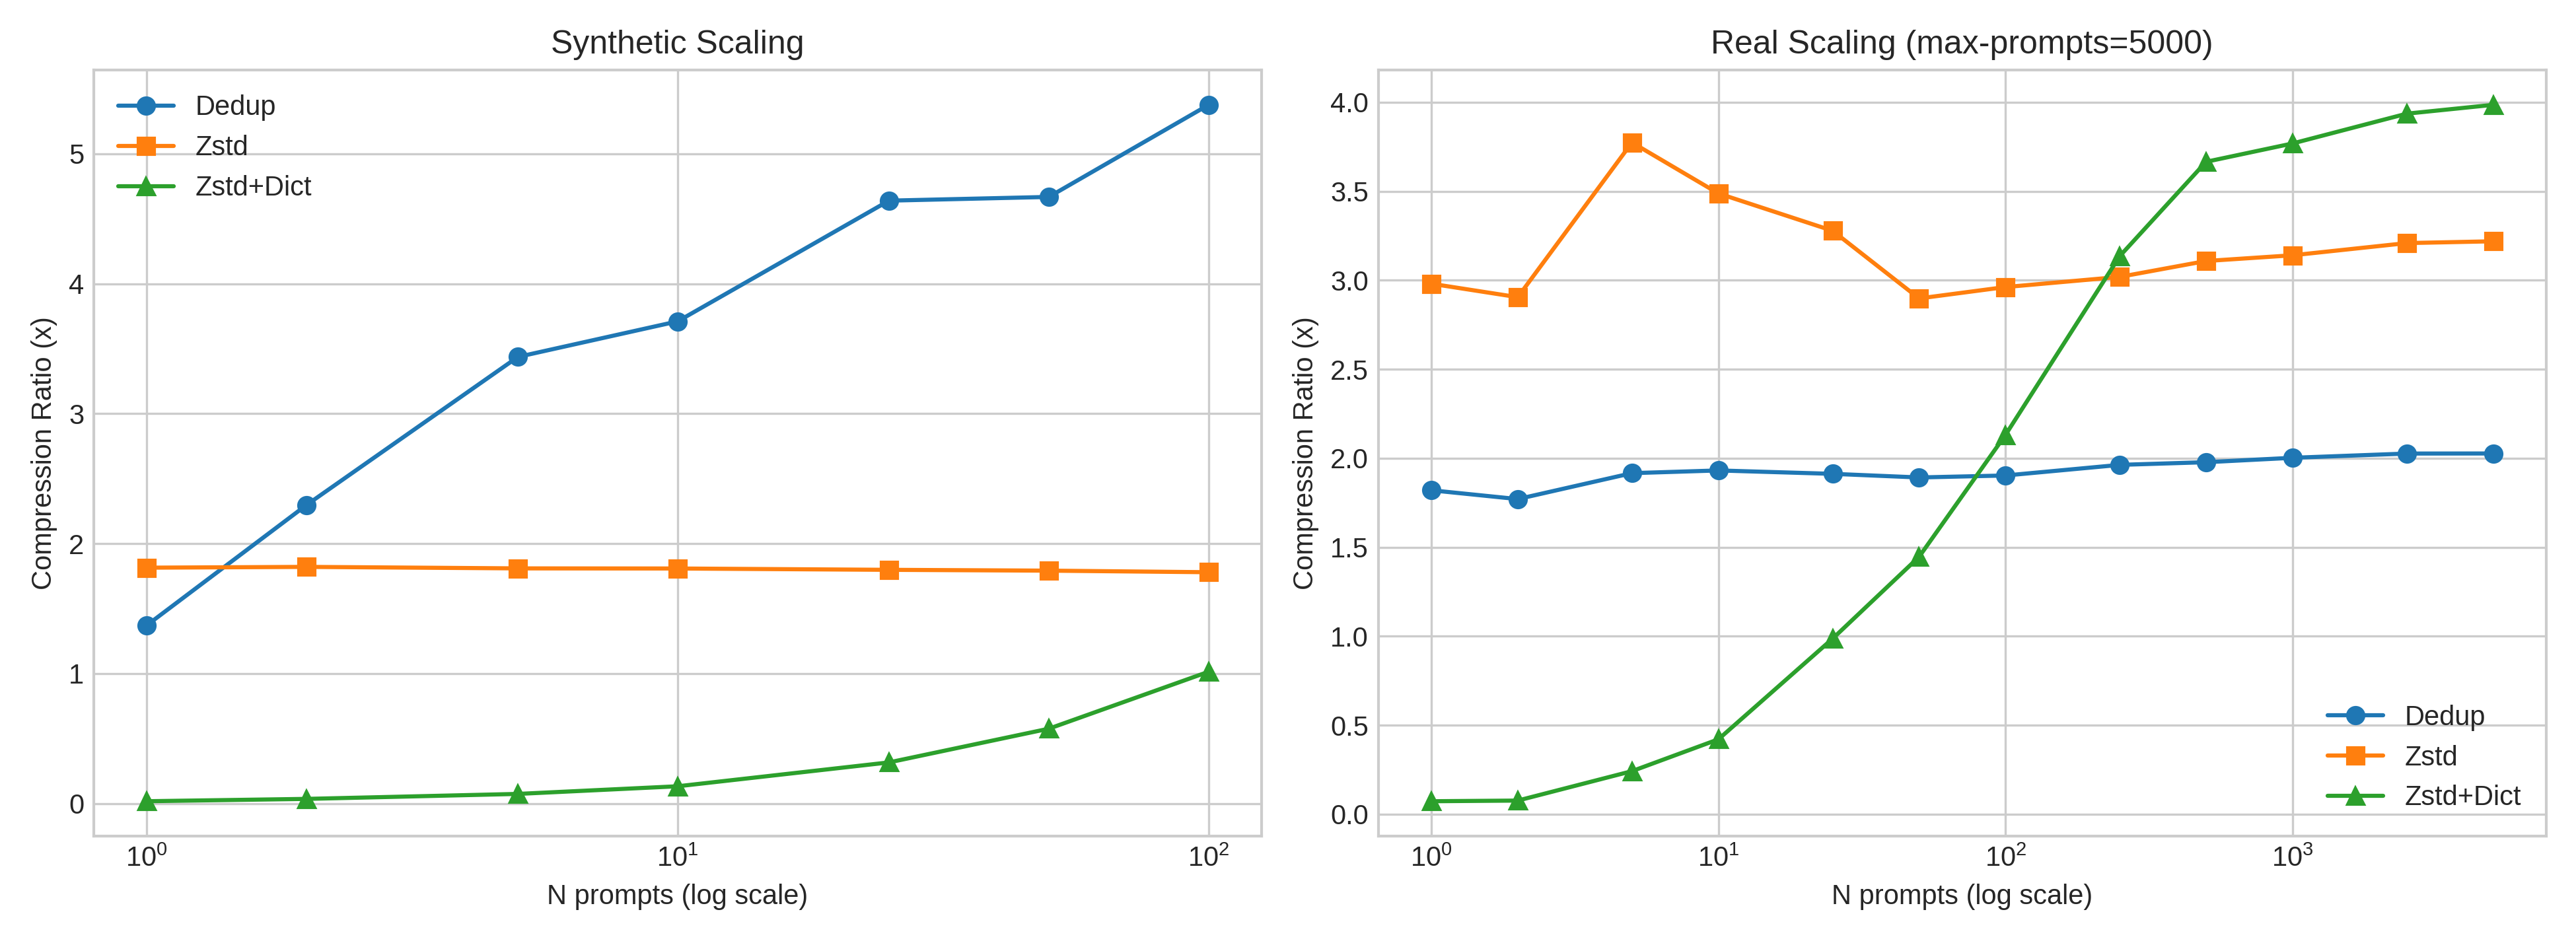
\includegraphics[width=\linewidth]{paper/figures/fig3_scaling_synthetic_real.png}
\caption{Fig3 Scaling Synthetic Real}
\label{fig:auto_fig3_scaling_synthetic_real}
\end{figure}

% Figure 4
egin{figure}[t]
\centering
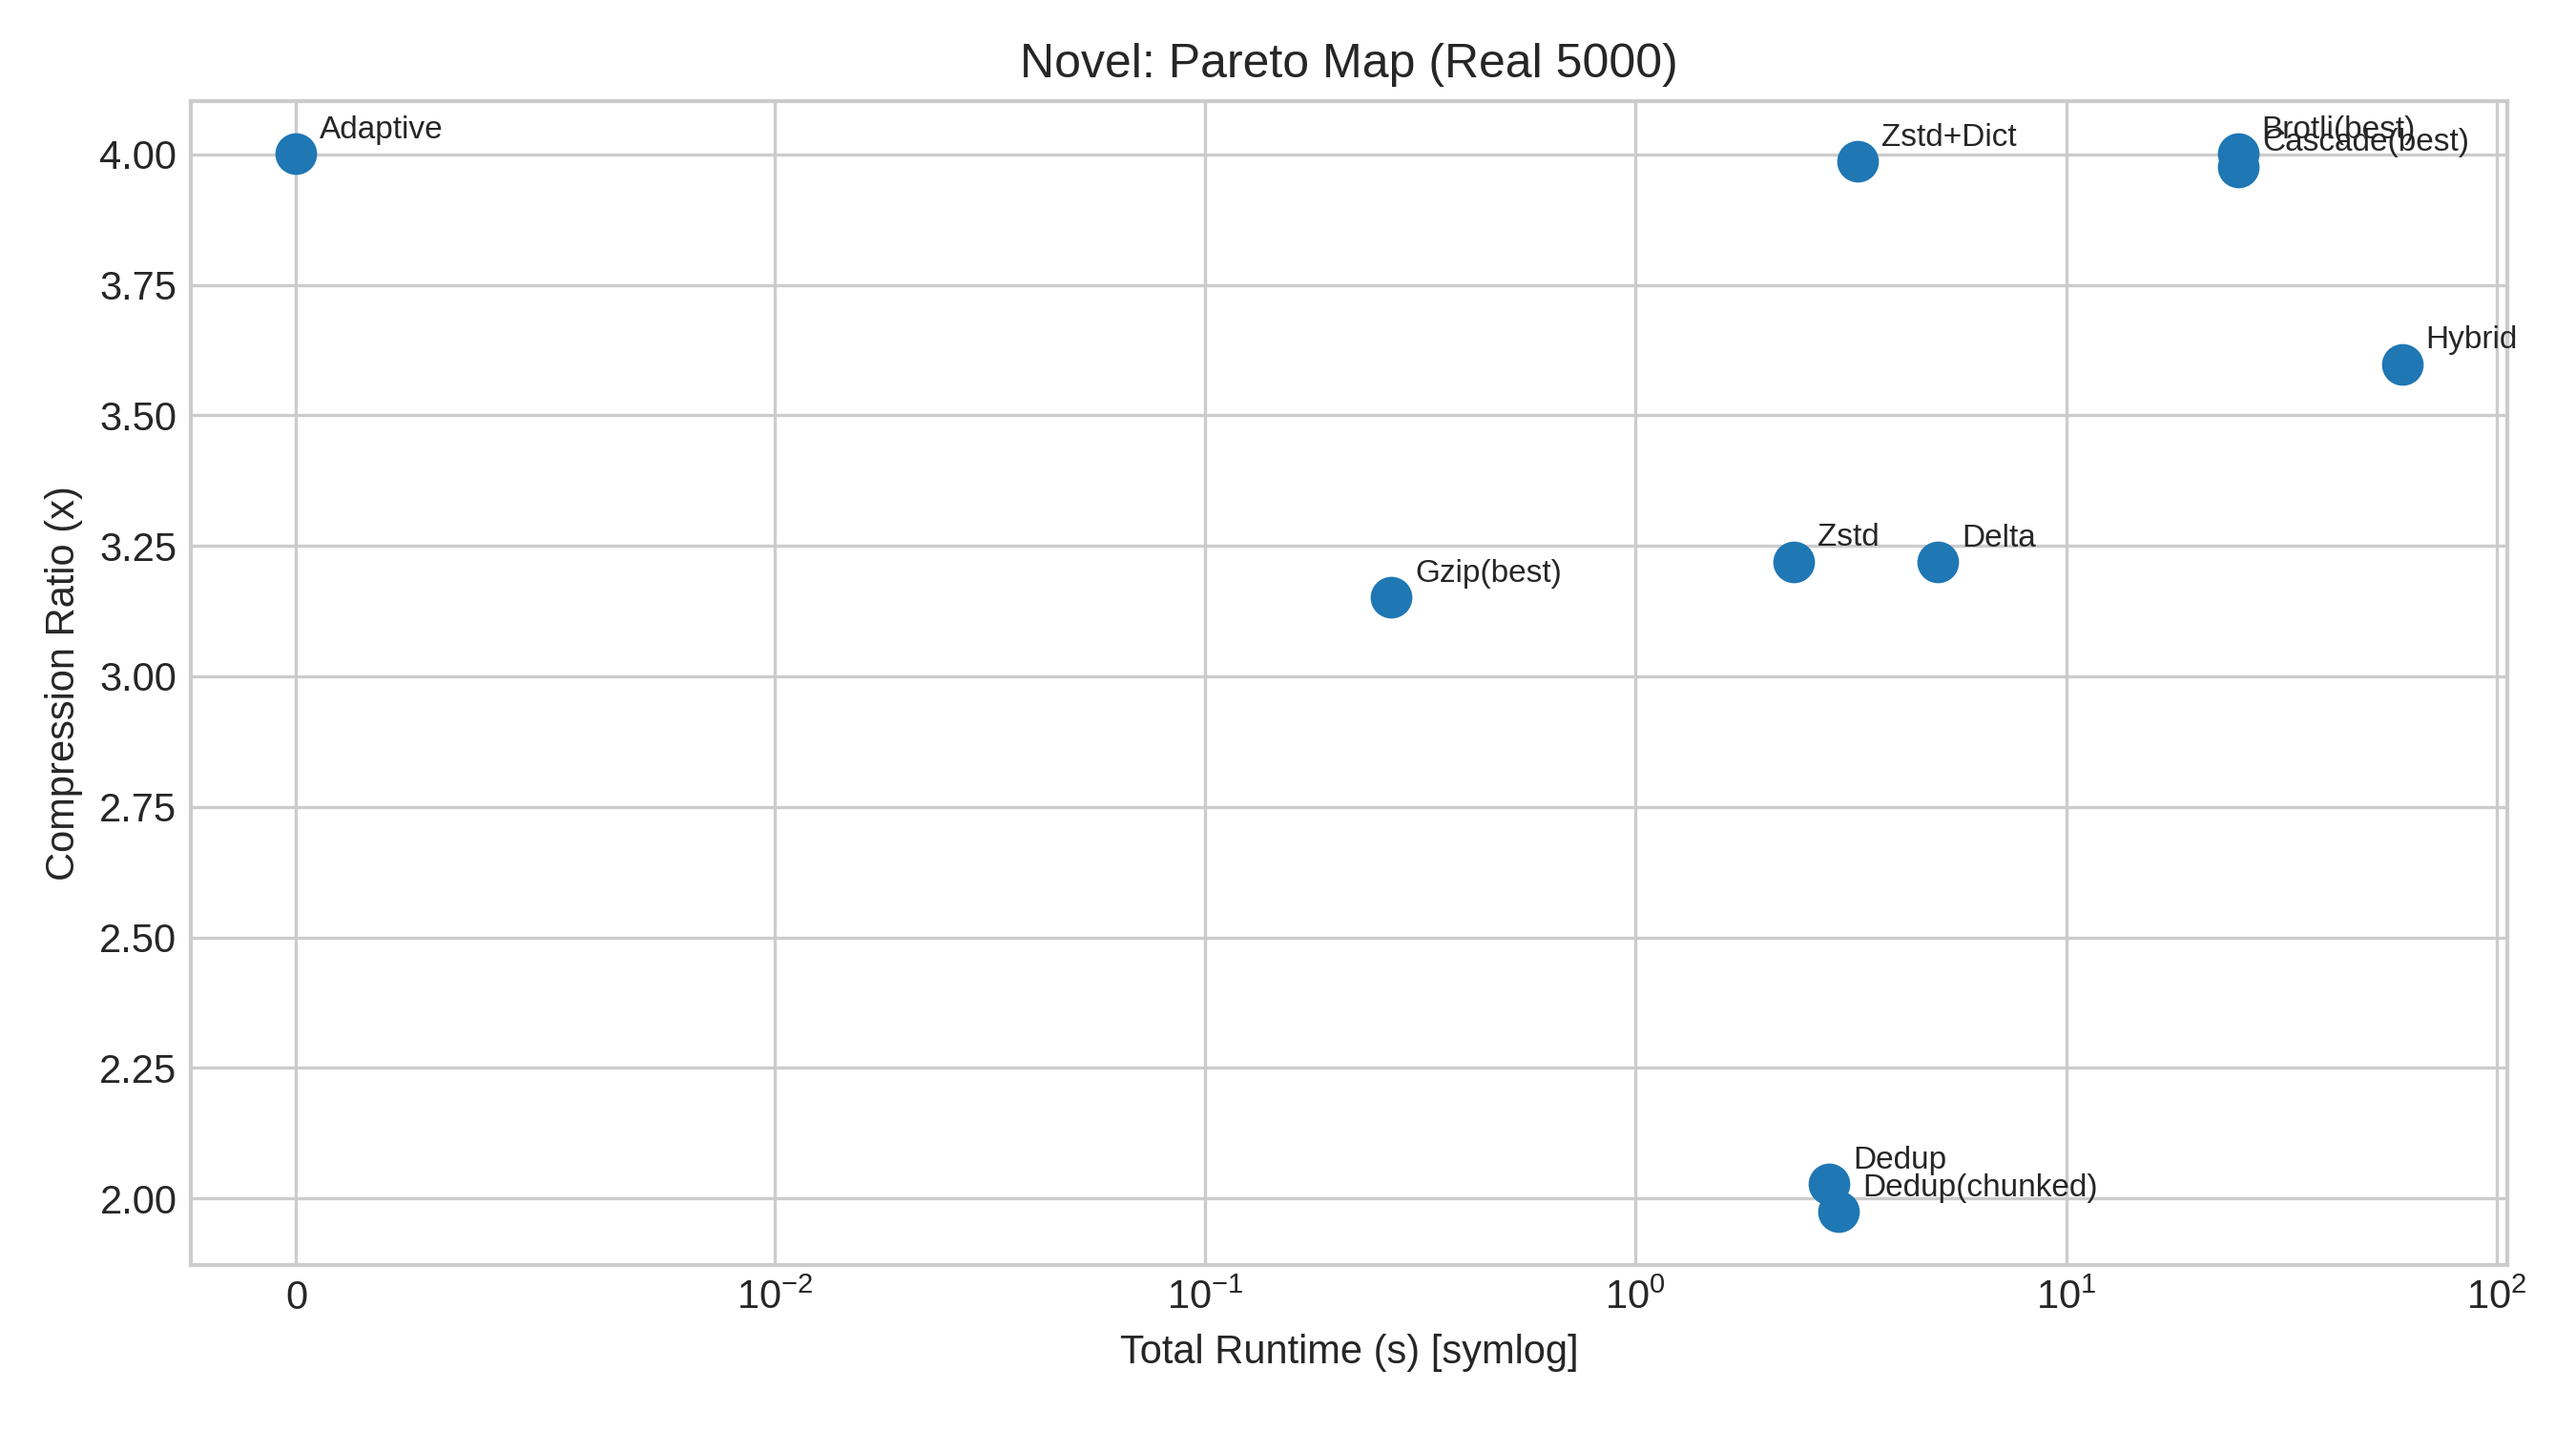
\includegraphics[width=\linewidth]{paper/figures/novel1_pareto_ratio_vs_time.png}
\caption{Novel1 Pareto Ratio Vs Time}
\label{fig:auto_novel1_pareto_ratio_vs_time}
\end{figure}

% Figure 5
egin{figure}[t]
\centering
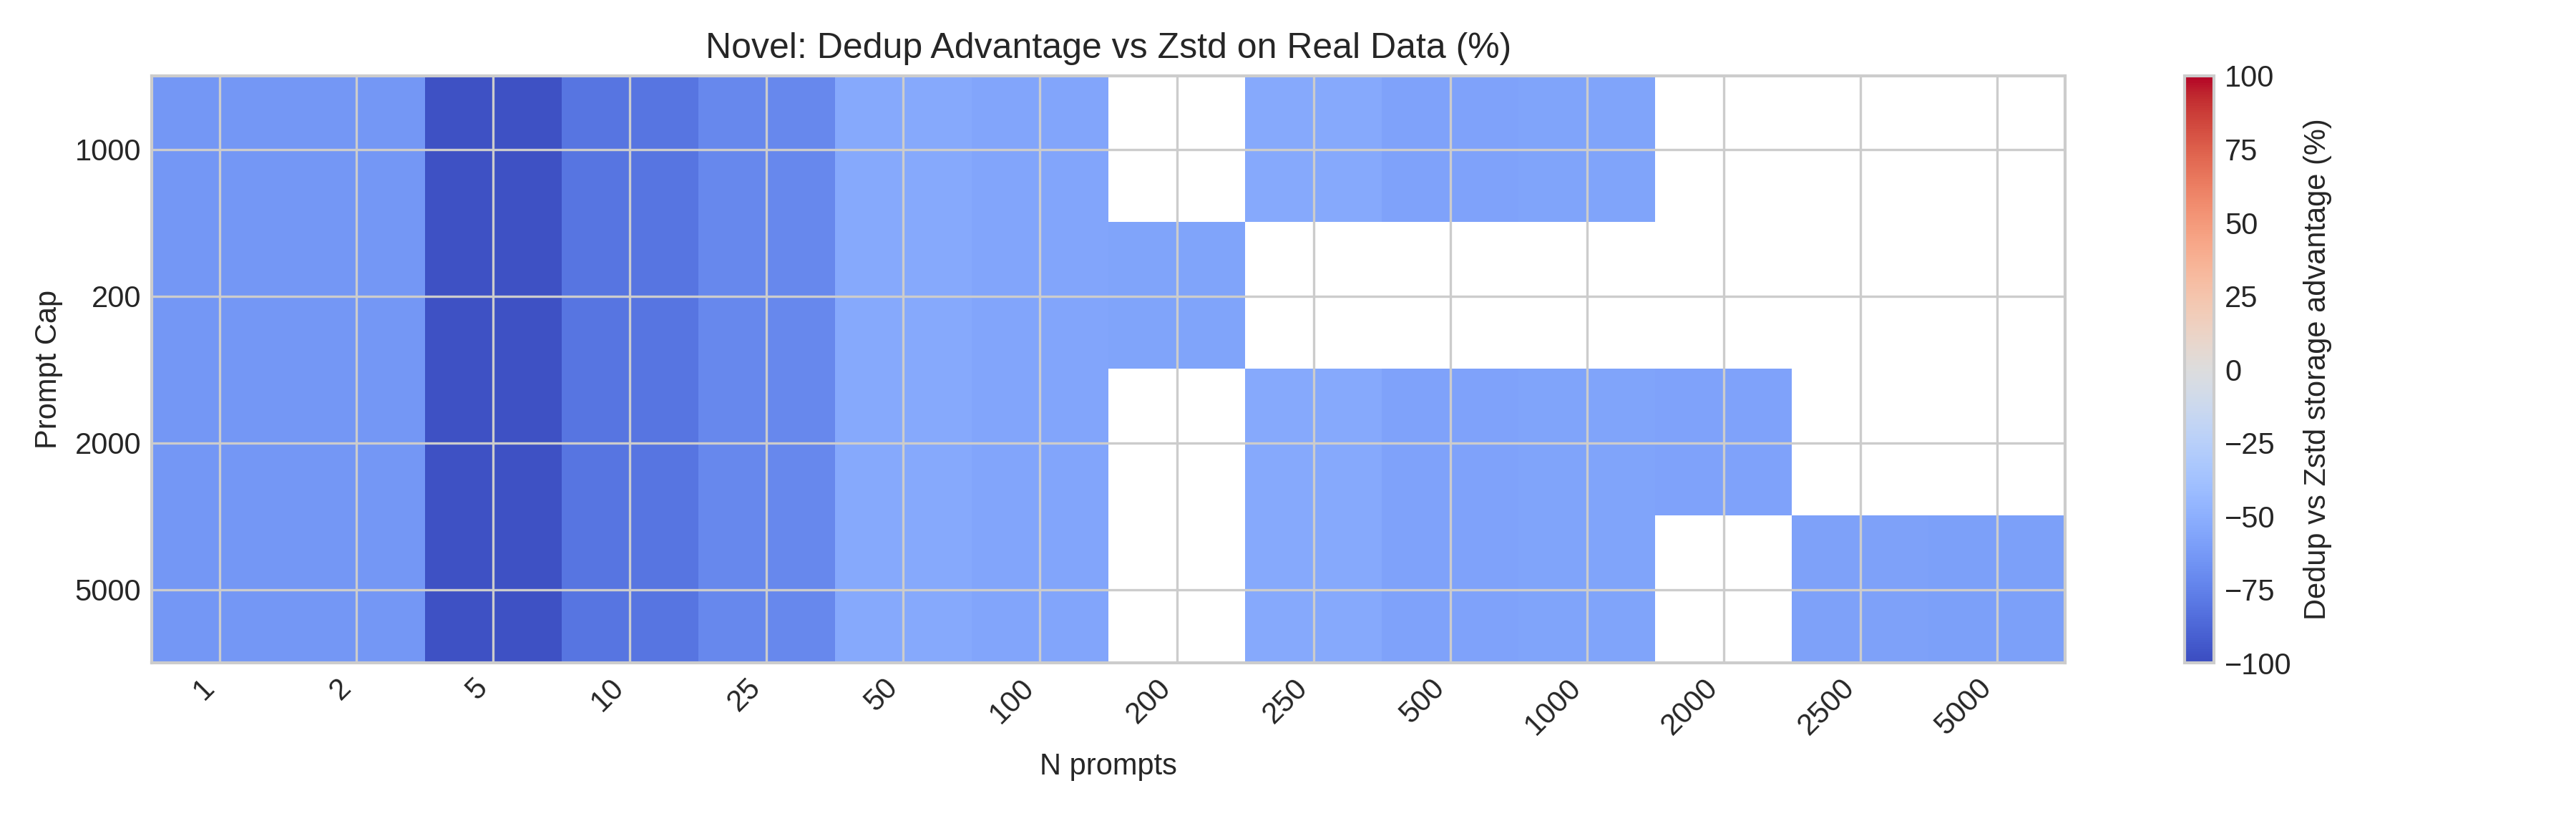
\includegraphics[width=\linewidth]{paper/figures/novel2_heatmap_dedup_advantage_real_caps.png}
\caption{Novel2 Heatmap Dedup Advantage Real Caps}
\label{fig:auto_novel2_heatmap_dedup_advantage_real_caps}
\end{figure}

% Figure 6
egin{figure}[t]
\centering
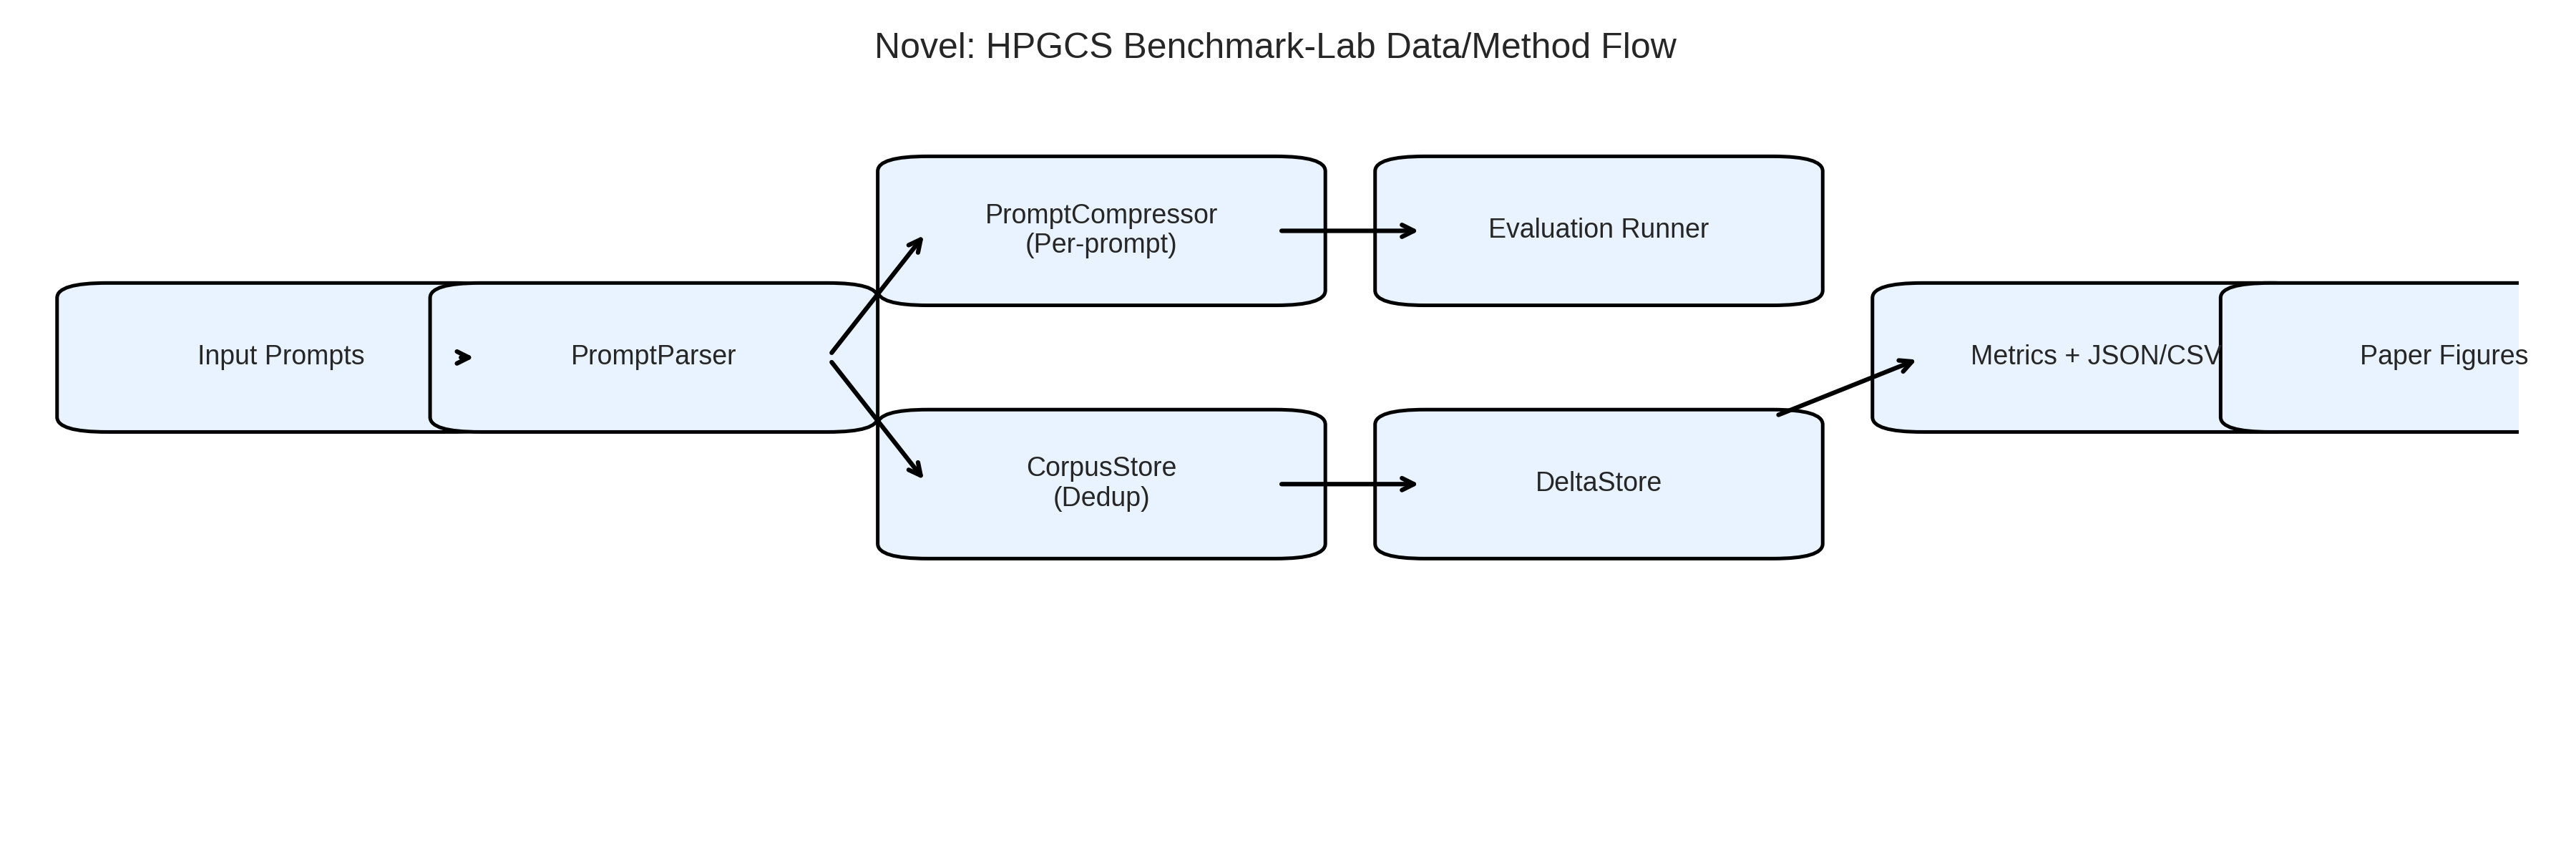
\includegraphics[width=\linewidth]{paper/figures/novel3_architecture_flow_diagram.png}
\caption{Novel3 Architecture Flow Diagram}
\label{fig:auto_novel3_architecture_flow_diagram}
\end{figure}
